% !TEX TS-program = pdflatex
% !TEX encoding = UTF-8 Unicode

% This is a simple template for a LaTeX document using the "article" class.
% See "book", "report", "letter" for other types of document.

\documentclass[11pt]{article} % use larger type; default would be 10pt

\usepackage[utf8]{inputenc} % set input encoding (not needed with XeLaTeX)

%%% Examples of Article customizations
% These packages are optional, depending whether you want the features they provide.
% See the LaTeX Companion or other references for full information.

%%% PAGE DIMENSIONS
\usepackage{geometry} % to change the page dimensions
\geometry{a4paper} % or letterpaper (US) or a5paper or....
% \geometry{margin=2in} % for example, change the margins to 2 inches all round
% \geometry{landscape} % set up the page for landscape
%   read geometry.pdf for detailed page layout information

\usepackage{graphicx} % support the \includegraphics command and options

% \usepackage[parfill]{parskip} % Activate to begin paragraphs with an empty line rather than an indent

%%% PACKAGES
\usepackage{booktabs} % for much better looking tables
\usepackage{array} % for better arrays (eg matrices) in maths
\usepackage{paralist} % very flexible & customisable lists (eg. enumerate/itemize, etc.)
\usepackage{verbatim} % adds environment for commenting out blocks of text & for better verbatim
\usepackage{subfig} % make it possible to include more than one captioned figure/table in a single float
% These packages are all incorporated in the memoir class to one degree or another...

%%% HEADERS & FOOTERS
\usepackage{fancyhdr} % This should be set AFTER setting up the page geometry
\pagestyle{fancy} % options: empty , plain , fancy
\renewcommand{\headrulewidth}{0pt} % customise the layout...
\lhead{}\chead{}\rhead{}
\lfoot{}\cfoot{\thepage}\rfoot{}

%%% SECTION TITLE APPEARANCE
\usepackage{sectsty}


\allsectionsfont{\sffamily\mdseries\upshape} % (See the fntguide.pdf for font help)
% (This matches ConTeXt defaults)

%%% ToC (table of contents) APPEARANCE
\usepackage[nottoc,notlof,notlot]{tocbibind} % Put the bibliography in the ToC
\usepackage[titles,subfigure]{tocloft} % Alter the style of the Table of Contents
\renewcommand{\cftsecfont}{\rmfamily\mdseries\upshape}
\renewcommand{\cftsecpagefont}{\rmfamily\mdseries\upshape} % No bold!

%%% END Article customizations


\usepackage[bulgarian]{babel}
\usepackage{physics}
\usepackage{amsmath}
\usepackage{centernot}
\usepackage{url}
\usepackage{graphicx}
\graphicspath{ {.} }
\usepackage{amsfonts}
\usepackage{xcolor}
\usepackage{enumitem}
\usepackage{systeme}


%%% The "real" document content comes below...

\title{26. Полиноми на една променлива. Теорема за деление с остатък. Най-голям общ делител на полиноми... }
\author{Play4u}
%\date{} % Activate to display a given date or no date (if empty),
         % otherwise the current date is printed
         

\newcommand{\lrangle}[1]{\left\langle #1 \right\rangle}

\newcommand{\oversetModels}[1]{\overset{#1}{\models}}

\newcommand{\italicBold}[1]{\textbf{\emph{#1}}}

\newcommand{\definition}{\italicBold{Дефиниция: }}
\newcommand{\theorem}{\italicBold{Теорема: }}
\newcommand{\lemma}{\italicBold{Лема: }}
\newcommand{\proof}{\italicBold{Доказателство: }}
\newcommand{\statement}{\italicBold{Твърдение: }}
\newcommand{\source}{\italicBold{Източник: }}

\newcommand{\redText}[1]{\textcolor{red}{#1}}

\newcommand{\curlies}[1]{\{#1\}}
\newcommand{\overbar}[1]{\mkern 1.5mu\overline{\mkern-1.5mu#1\mkern-1.5mu}\mkern 1.5mu}

\newcommand{\enumNum}{\renewcommand{\theenumi}{\arabic{enumi}}}
\newcommand{\enumlet}{\renewcommand{\theenumi}{\alph{enumi}}} 

\begin{document}
\maketitle

\italicBold{Конспект: } Във въпроса се включва определение на полином с коефициенти над поле, степен на полином и корени на полиноми. Теорема за деление с остатък. Схема на Хорнер. Всеки идеа в $F[x]$ е главен. Принцип за сравняване на коефициенти. Определение на най-голям общ делител на два полинома НОД $(h(x),g(x)) = (h(x), g(x))$, теорема за съществуване на най-голям общ делител на два полинома с коефициенти над поле, изразяване на $h(x),g(x)$ чрез полиномите $h(x)$ и $g(x)$(тъждество на Безу), алгоритъм на Евклид. Корени на полиноми. Формули на Виет.

\section{Полиноми на една променлива}
\italicBold{Източник: \path{https://store.fmi.uni-sofia.bg/fmi/algebra/lect_notes_nenov/08.pdf}}\\\par

\definition Нека $K$ е пръстен. Полином на променлива $x$ над пръстена $K$, наричаме израз от вида: \\
\centerline{$f(x) = a_{0}x^{0} + a_{1}x^{1} + a_{2}x^{2} + ... + a_{n}x^{n}$,}
където $a_{0}, a_{1},...,a_{n} \in K$ и се наричат коефициенти на $f(x)$.\\\par

\definition Ако всияки коефициенти на $f(x)$ са равни на 0, $f(x)$ се нарича нулев полином. \\\par

\definition Степен на полином: Ако $f(x)$ е ненулев полином, тогава най-голямото естествено число $n$, за което коефициентът пред $x^{n}$ във $f(x)$ е различен от нула се нарича \textit{степен на } $f(x)$ и се бележи със ст.$(f(x))$  или $deg(f(x))$. Единствено нулевият полином няма определена степен. \\\par

\definition Корени на полином: Нека $K$ е пръстен и $f(x) \in K[x]$. Нека $\alpha \in K$ и $f(x) = a_{0} + a_{1}x + a_{2}x^{2}+...+a_{n}x^{n} \in K[x]$. Тогава $f(\alpha) = a_{0} + a_{1}\alpha + a_{2}\alpha^{2}+...+a_{n}\alpha^{n} \in K$ се нарича стойност на $f(x)$ при $x = \alpha$. Ако $f(\alpha) = 0$, казваме че $\alpha$ е \textit{корен} на $f(x)$.

\section{Делимост на полиноми}
\italicBold{Източник: \path{https://debian.fmi.uni-sofia.bg/study/materials/va/lectures/9.pdf}}\\\par

\definition(За делимост с остатък) Нека $F$ е поле. За всеки два полинома $f(x), g(x) \in F[x], g(x) \neq 0$ съществуват единствени полиноми $q(x) \in F[x]$, наречен частно и $r(x) \in F[x]$, наречен остатък, че е изпълнено \\
\centerline{$f(x) = q(x)g(x) + r(x)$}
и $deg(r)<deg(g)$

\italicBold{Схема на Хорнер}\\
\italicBold{Източник: \path{https://debian.fmi.uni-sofia.bg/study/materials/va/exercises/4.pdf}}\\

Нека е даден полинома\\
\centerline{$f(x)=a_{0}x^{n}+a_{1}x^{n-1}+...+a_{n-1}x+a_{n}$}
над някакво поле. Нека да го разделим с частно и остатък на полинома от първа степен $x - \alpha$, където $\alpha$ е елемент от полето. Тогава частното е полином от $n-1$ степен и можем да го запишем\\

\centerline{$a_{0}x^{n}+...+a_{n}=(x-\alpha)(b_{0}x^{n-1}+b_{1}x^{n-2}+...+b_{n-2}x+b_{n-1})+b_{n}$,}

където остатъкът $b_{n}$ е елемент от полето, понеже според теоремата за деление, неговата степен е или 0 или $-\infty$. Ясно е, че $\alpha$ е корен на $f(x)$ точно когато $b_{n} = f(\alpha) = 0$. От принципа за сравняване на коефициентите имаме \\

\begin{center}\begin{tabular}{ccl}\
$a_{0}$ & = & $b_{0}$, \\
$a_{1}$ & = & $b_{1}-\alpha b_{0}$, \\
... \\
$a_{n-1}$ & = & $b_{n-1}-\alpha b_{n-2}$, \\
$a_{n}$ & = & $b_{n}-\alpha b_{n-1}$, \\
\end{tabular}\end{center}

откъдето всъщност изразяваме коефициентите $b_{i}$ като \\
\begin{center}\begin{tabular}{ccl}\
$b_{0}$ & = & $a_{0}$, \\
$b_{1}$ & = & $\alpha b_{0} + a_{1}$ \\
... \\
$b_{n-1}$ & = & $\alpha b_{n-2} + a_{n-1}$ \\
$b_{n}$ & = & $\alpha b_{n-1} + a_{n}$ \\
\end{tabular}\end{center}

Тези резултати обикновено се записват в таблица\\ 
\begin{center}
	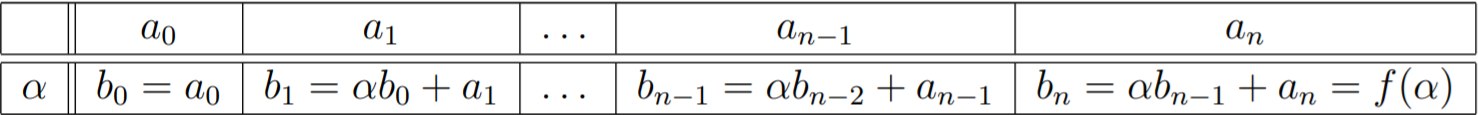
\includegraphics[scale=0.45]{Horner.png}
\end{center}
наречена схема на Хорнер. Ако решим да приложим схемата на Хорнер върху получения полином $b_{0}x^{n-1}+...+b_{n-1}$, то просто прилагаме същия метод, използвайки числата получени в предходния ред на таблицата, за да попълним текущия ред. \\\par

\statement Всеки идеал във $F[x]$ е главен.\\
\source \path{http://fmi.wikidot.com/alg214#toc8}\\

Нека $F$ е поле. Нека $I \triangleleft$ $F[x]$($I$ е идеал на пръстена на полиномите над полето $F$). Тогава $\exists f \in F[x]: I = (f(x))$ (съшествува елемент, който поражда идеала), или иначе казано: всеки идеал на пръстена на полиномите над дадено поле е главен.\\

\proof (\italicBold{Опционално:? })\\

\enumNum
\begin{enumerate}
	\item $I = \curlies{0} \rightarrow I = (0)$ - вярно \\
	\item $I \neq \curlies{0}$\\
\end{enumerate}
Нека $0 \neq d(x) \in I$ е полиномът с най-ниска степен. Нека $f(x) \in I$ е произволен. Разделяме $f(x)$ с частно и остатък на $d(x)$\\
\centerline{$f(x) = q(x)d(x)+r(x), deg(r) < deg(d)$}
$\rightarrow r(x) = \underbrace{f(x)}_{\in I}-\underbrace{d(x)q(x)}_{\in I} \rightarrow r(x)\in I$
Тъй като $d(x)$ е с минимална степен, а $deg(r) < deg(d)$ и $r \in I$, то $r(x) = 0$\\
$\rightarrow f(x)=q(x)d(x)\rightarrow f(x) \in ((dx)) \rightarrow I \subset (d(x))$\\
$\rightarrow I = (d(x))$\\
\textbf{Ако $F$ не е поле, твърдението не е вярно!}\\\par

\definition Принцип за сравняване на коефициентите\\
\source \path{http://fmi.wikidot.com/alg214#toc8}\\
Нека $F$ е поле.\\
Нека $f(x), g(x) \in F[x], deg(f) \leq n, deg(g) \leq n$\\
Ако $a_{1}, a_{2},..., a_{n}, a_{n+1} \in F$ са две по две различни поможеду си(т.е. $a_{i} = a_{j} \leftrightarrow i=j$)и такива, че: \\

\centerline{$f(a_{i}) = g_(a_{i}), 1 \leq i \leq n+1$, то $f(x) = g(x)$}

Или иначе казано, ако за два полинома със степени не по-големи от дадено фиксирано число $n$(най-често $n$ е по-голямата от двете степени), намерим $n+1$ числа, такива, че стойностите на полиномите са равни, то те изцяло съвпадат.\\
Или иначе казано, полином от степен $n$ се дефинира от $n+1$ точки.\\
\centerline{Insert proof here}\\\par

\definition НОД\\
\source \path{https://store.fmi.uni-sofia.bg/fmi/algebra/lect_notes_nenov/11.pdf}\\

Нека $K$ е комутативен пръстен и $f(x), g(x) \in K[x]$. Най-голям общ делител(НОД)на $f(x)$ и $g(x)$ в пръстена $K[x]$ наричаме такъв полином $d(x) \in K[x]$, че:

\enumNum
\begin{enumerate}
	\item $d(x)$ дели $f(x)$ и $g(x)$;\\
	\item ако $d_{1}$ дели $f(x)$ и $g(x)$, тогава $d_{1}(x)$ дели $d(x)$ \\\par
\end{enumerate}

\theorem Нека $F$ е поле. ТОгава всеки два полинома от $F[x]$ имат НОД във $F[x]$\\
\proof \\
Нека $f(x), g(x) \in F[x]$. Ако $f(x) = g(x) = 0$, тогава НОД е нулевият полином(в тази ситуация всеки поином от $F[x]$ е обю делите на $f(x)$ и $g(x)$), но единствено нулевият полином удолетворява второто условие за НОД). Поради това ще предполагаме, че \\
\centerline{(\#)Поне единият от $f(x), g(x)$ е ненулев}
Дефинираме \\

\centerline{$S = \curlies{M(x)f(x)+N(x)g(x)|M(x),N(x)\in F[x]}$}

Като положим $N(x) = 0$ и $M(x) = 1$ получаваме $f(x) \in S$, а като положим $N(x) = 1$ и $M(x) = 0$ получаваме $g(x) \in S$. Следователно $f(x), g(x) \in S$. От (\#) става ясно, че в $S$ има ненулеви полиноми. Измежду всички ненулеви полиноми в $S$ избираме такъв ненулев полиним $d(x)$, който има най-ниска възможна степен. Имаме\\

\centerline{(\#\#)$deg(d(x)) \leq deg(h(x))$, за всеки ненулев $h(x) \in S$}

От $d(x) \in S$ следва \\

\centerline{(\#\#\#)$d(x) = M_{0}(x)f(x)N_{0}(x)g(x)$}

Ще докажем, че $d(x)$ е НОД на $f(x)$ и $g(x)$. Понеже $S \subseteq F[x], d(x) \in F[x]$.

\enumNum
\begin{enumerate}
	\item Защо $d(x)$ е общ делител на $f(x)$ и $g(x)$?\\
		Допускаме, че $d(x)$ не дели $f(x)$. Тогава $f(x) = d(x)q(x) + r(x)$, където $r(x) \neq 0$ и $deg(r(x)) < deg(d(x))$. Като използваме (\#\#\#) получаваме \newpage
		
		\centerline{$r(x) = f(x)-d(x)q(x)=f(x)-(M_{0}(x)f(x)+N_{0}(x)g(x))q(x)=$}
		\centerline{$=\underbrace{(1-M_{0}(x)q(x))}_{M(x)}f(x)-\underbrace{N_{0}(x)q(x)}_{N(x)}g(x)$}
		Следователно, $r(x)=M(x)f(x)+N(x)g(x)$ и поради това $r(x)\in S$. Полиномът $r(x)$ принадлежи на множеството $S$ и има степен по-малка от $d(x)$, което противоречи на (\#\#). Това противоречие доказва, че $d(x)$ дели $f(x)$. По същият начин се доказва, че $d(x)$ дели $g(x)$\\
	\item Нека $d_{1}(x)$ дели $f(x)$ и $g(x)$. От (\#\#\#) следва, че $d_{1}(x)$ дели $d(x)$.\\
	Теоремата е доказана\\\par
\end{enumerate} 

\theorem (\textbf{Теорема на Безу})\\
\source \path{http://fmi.wikidot.com/alg201#toc7}\par

Нека $a,b \in \mathbb{Z}$ като $a \neq 0$ или $b \neq 0$. Тогава $\exists!d=(a,b)$ и $d = ua + vb$, където $u, v \in \mathbb{Z}^{3}$(тъждество на Безу).\\

\proof (\textbf{Опционално:?})\\
Разглеждаме множеството $M = \curlies{xa + yb|x,y \in Z}$.\\
Вземаме неговото подмножество $M^{+}=\curlies{z \in M|z>0}\neq \emptyset$.\\
$M^{+}\subset \mathbb{N} \rightarrow \exists d$ - минимален елемент в $M^{+}$.\\
$d = x_{1}a+y_{1}b > 0$\\
Нека $c \in M$. Тогава $c = x_{2}a + y_{2}b$ (от дефиницията на $M$).\\
От друга страна, ако използваме теоремата за деление с частно и остатък за $c$ и $d$ получаваме\\
$c = dq+r, 0\leq r < |d| = d$\\
Сега да използваме двете представяния на $c$:\\
$x_{2}a+y_{2}b=c=dq+r=(x_{1}a+y_{1}b)q+r$\\
От тук получихме формулата за $r:r=(x_{2}-x_{1}q)a+(y_{2}-y_{1}q)b$.\\
Очевидно $r \in M$ и е неотрицателно(от теоремата за деление с частно и остатък). Също така $r < d$ следователно не е от $M^{+}$(защото $d$ е минимален елемент) и остана $r=0$. Така получихме, че $d / c$.\\
Ще докажем, че $d$ е НОД на $a,b$:\\

\enumNum
\begin{enumerate}
	\item Ако $c \in M \rightarrow d / c$. Сега понеже $a,b \in M$ имаме $d / a \;\&\; d / b$, т.е. $d$ е техен общ делител.\\
	\item Нека $d_{1}$ е произволен общ делител на $a,b$. Тогава $d_{1} / a \;\&\; d_{1} / b$, следователно $d_{1} / \underbrace{x_{1}a+y_{1}b}_{d} $. Т.е. получихме, че $d_{1} / d$. \\ 
\end{enumerate}
Следователно, по дефиниция за НОД $: d = (a,b)$\\\par

\italicBold{Алгоритъм на евклид за намиране на полиноми}\\
\source \path{http://fmi.wikidot.com/alg201#toc7}\\
\textbf{Дадено: } $a, b \in \mathbb{Z}, a,b \neq 0$\\
\textbf{Резултат: } $d=$ НОД$(a,b)$.\\
\textbf{Процедура: }\\
От теоремата за деление с частно и остатък $\rightarrow a=bq_{1}+r_{1}, 0 \leq r_{1} < |b|$.\\
Първо ще докажем, че НОД($a, b$) = НОД($b, r_{1}$).\\
Нека $d_{1}=(a,b)$ и $d_{2}=(b, r_{1})$\\
Ot $d_{1}$ = НОД$(a,b) \rightarrow d_{1}|a$ и $d_{1}|b \rightarrow d_{1}|(a-bq_{1})\rightarrow d_{1}|r_{1}$\\
$\rightarrow d_{1}|d_{2}$(1)\\
От $d_{2}$ = НОД$(b, r_{1}) \rightarrow d_{2}|b_{2}$ и $d_{2}|r_{1} \rightarrow d_{2}|(bq_{1}+r_{1})\rightarrow d_{2}|a$\\
$\rightarrow d_{2}|d_{1}$(2)\\
От (1) и (2) $\rightarrow d_{1} = d_{2}$.\\
До тук: $a = bq_{1} + r_{1}$ и $(a,b) = (b, r_{1})$\\
Ако $r_{1} = 0 \rightarrow d= b$ - търсеният НОД.\\
Иначе(ако $r_{1}\neq 0$), то $b = r_{1}q_{2}, 0 \leq r_{2}<r_{1}$ като $(b, r_{1}) = (r_{1}, r_{2})$.\\
Отново, ако $r_{2} = 0 \rightarrow d = r_{1}$;\\
иначе: процесът се повтаря.\\
Знаем, че за НОД$(a,b)$ можем да получим минимум 1, т.е. процесът е краен.\\
На $k$-тата стъпка имаме:\\
$r_{k-1}=r_{k}q_{k+1}+r_{k+1},0 \leq r_{k+1} < r_{k}$ и $(r_{k-1}, r_{k}) = (r_{k}, r_{k+1})$.\\
$|b|>r_{1}>r_{2}...>r_{k-1}>r_{k}>...\geq 0$\\
На $(k+1)$-ва стъпка получаваме следното:\\
$r_{k} = r_{k+1}q_{k+2}+0$ и $(r_{k}, r_{k+1})=(r_{k+1},0)=r_{k+1}$\\
Тъй като $(a,b)=(b,r_{1})=(r_{1}, r_{2})=...=(r_{k-1}, r_{k})=(r_{k},r_{k+1})=r_{k+1}$.\\\\
\noindent НОД$(a,b)=r_{k+1}$ \\

\section{Корени на полиноми. Формули на Виет}
\source \path{http://fmi.wikidot.com/alg217#toc2}\\

\definition Корен на полином:\\
Нека $f(x) \in F[x]$ е произволен полином. $\alpha \in F$ наричаме корен на полинома $f(x)$, ако е изпълнено, че:\\
\centerline{$f(\alpha) = 0$}
Това е равносилно на $x-\alpha|f(x)$. Проверява се тривиално с теоремата за деление с частно и остатък. \\\par

\definition \italicBold{Опционално?: }$K$-кратен корен:\\
Нека $f(x) \in F[x]$ e произволен полином. Казваме, че $\alpha \in F$ е $k$-кратен корен на полинома $f(x)$, ако е изпълнено, че:

$
   \left\{\begin{aligned}
    (x-\alpha)^{k} & \;\;|& f(x)\\
    (x-\alpha)^{k+1} & \not|& f(x)\\
   \end{aligned}\right.
$\\\par


\subsection{Формули на Виет}
Ще напишем формули, които свързват корените на даден полином с неговите коефициенти.\\

\theorem Формули на Виет:\\
Нека $f(x) = a_{0}x^{n}+a_{1}x^{n-1}+...+a_{n-1}x+a_{n}$ е произволен полином от $F[x]$.\\
Нека $\beta^{1}, \beta^{2},...,\beta^{n}$ са всичките му корени в някакво разширение $K \supset F$. Тогава:

\begin{center}\begin{tabular}{cccl}\
$\Sigma_{i}\beta_{i}$ & = & $\beta_{1}+\beta_{2}+...+\beta_{n}$ & =  $-\frac{a_{1}}{a_{0}}$ \\
$\Sigma_{i<j}\beta_{i}\beta_{j}$ & = & $\beta_{1}\beta_{2}+\beta_{1}\beta_{3}+...+\beta_{1}\beta_{n}+\beta_{2}\beta_{3}+...+\beta_{n-1}\beta_{n}$ & = $\frac{a_{2}}{a_{0}}$\\
\vdots\\
$\prod_{i}\beta_{i}$ & = & $\beta_{1}\beta_{2}...\beta_{n}$ & =
$(-1)^{n}\frac{a_{n}}{a_{0}}$\\\\\par

\centerline{\textit{Insert proof here}}
 
\end{tabular}\end{center}


\end{document}





